\chapter{Getting Started}
\section{Installation}
At this moment in time installation is pretty basic, we have not packaged the program in any way.  So, for now, the best way to install is to download the programs, install them somewhere appropriate, and run them with Python 3.7.
 
\section{First run}
When the program is run for the first time it will create a database, because one does not exist, and will present the screen shown in Figure \ref{fig:firstrun}.
\begin{figure}[h]
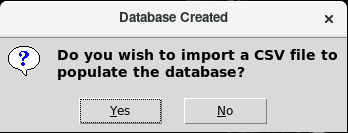
\includegraphics[scale=1]{firstRun.png}
\caption{First run, database creation}
\label{fig:firstrun}
\end{figure}
For now we will assume that you do not have an available CSV file in the correct format (more on this in Section \ref{sect:csv}), and you select \textbf{\textit{No}}

\section{Start screen}
Once past the first run screen, or if this is not the first time you have run the program, you will see the screen shown in Figure \ref{fig:firstscreen}. Which, of course, would ordinarily be populated with elements of your music library.
\begin{figure}[h]
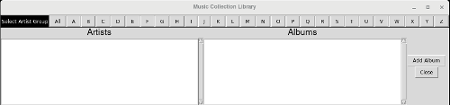
\includegraphics[width=\textwidth]{firstScreen.png}
\caption{Start screen}
\label{fig:firstscreen}
\end{figure}
The main areas of interest are:

\subsection{The artist selection bar}
The Artist selection bar, see Figure \ref{fig:artistselectionbar}, allows you to select a group of artists whose sort criteria begin with a specific letter of the alphabet.  The default selection is \textbf{\textit{All}}.
\begin{figure}[h]
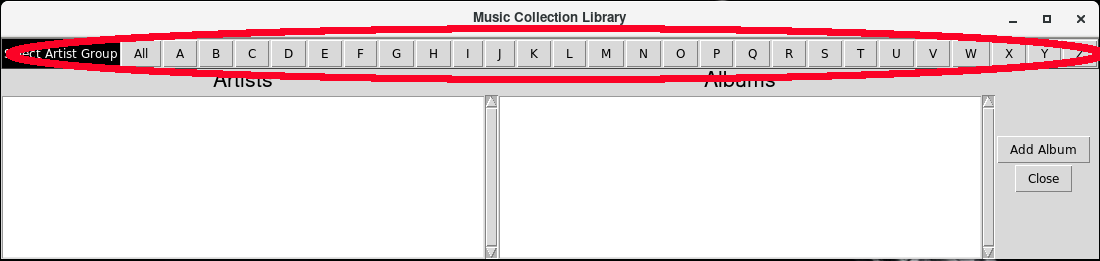
\includegraphics[width=\textwidth]{artistSelectionBar.png}
\caption{Artist Selection bar}
\label{fig:artistselectionbar}
\end{figure}

\subsection{The add album button}
The \textbf{\textit{Add Album}} button, as shown in Figure \ref{fig:addalbumbutton}, allows the adding of album data.  More of which in Section \ref{sect:albums}.
\begin{figure}[h]
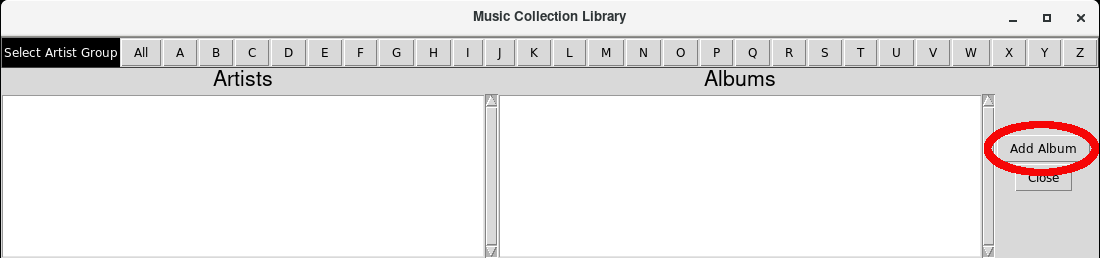
\includegraphics[width=\textwidth]{albumButton.png}
\caption{Add album button}
\label{fig:addalbumbutton}
\end{figure}

\subsection{The close button}
The \textbf{\textit{Close}} button, as shown in Figure \ref{fig:closebutton}, exits the program.
\begin{figure}[h]
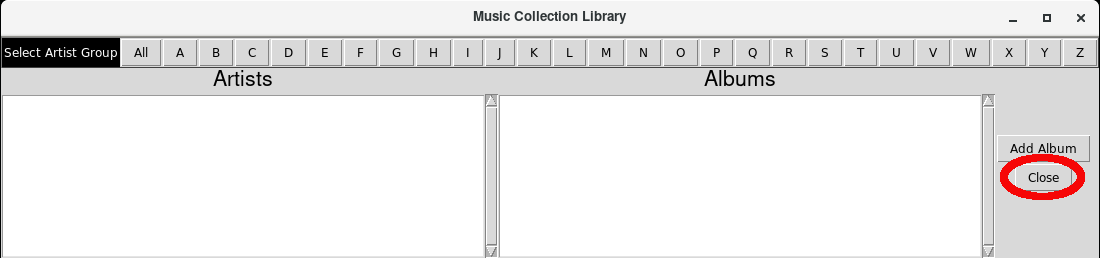
\includegraphics[width=\textwidth]{closeButton.png}
\caption{Close button}
\label{fig:closebutton}
\end{figure}